\documentclass{article}
\usepackage{amsmath}
\usepackage{amssymb}
\usepackage{tikz}
\usetikzlibrary{positioning}

\begin{document}

\begin{figure}[h]
    \centering
    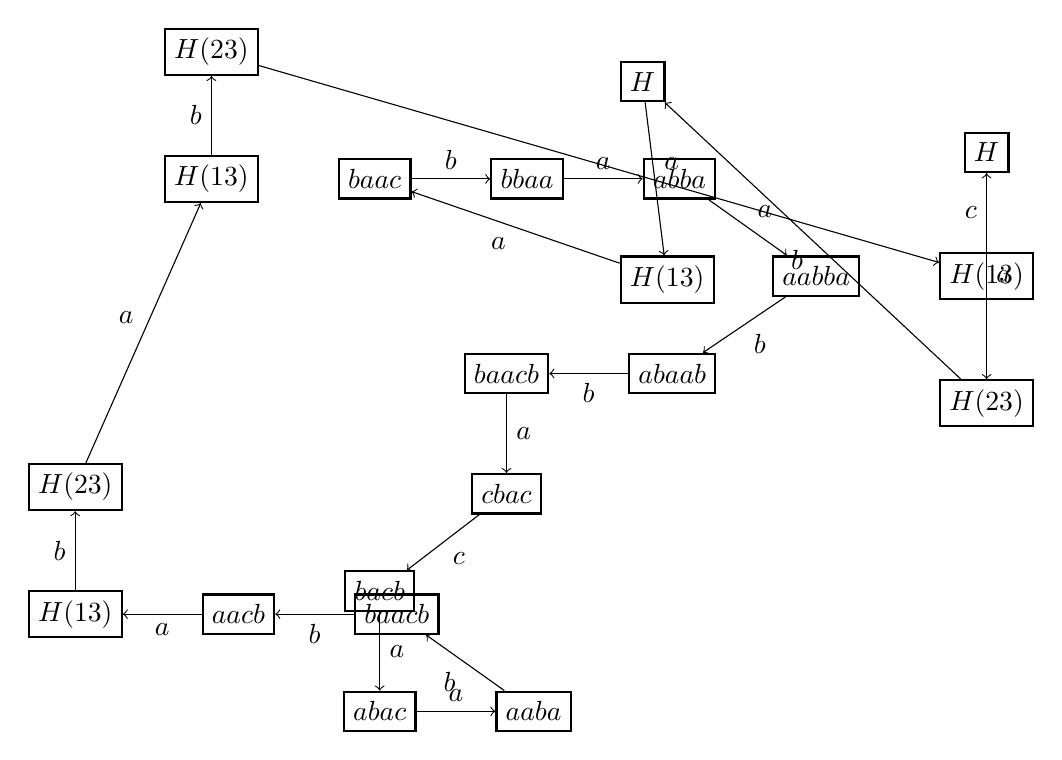
\begin{tikzpicture}[node distance=1cm, auto]
        \tikzstyle{state}=[rectangle, draw=black, thick, minimum size=0.5cm]

        % Define nodes
        \node[state] (A) {$baac$};
        \node[state] (B) [right=of A] {$bbaa$};
        \node[state] (C) [right=of B] {$abba$};
        \node[state] (D) [below right=of C] {$aabba$};
        \node[state] (E) [below left=of D] {$abaab$};
        \node[state] (F) [left=of E] {$baacb$};
        \node[state] (G) [below=of F] {$cbac$};
        \node[state] (H) [below left=of G] {$bacb$};
        \node[state] (I) [below=of H] {$abac$};
        \node[state] (J) [right=of I] {$aaba$};
        \node[state] (K) [above left=of J] {$baacb$};
        \node[state] (L) [left=of K] {$aacb$};
        \node[state] (M) [left=of L] {$H(13)$};
        \node[state] (N) [above=of M] {$H(23)$};
        \node[state] (O) [left=of A] {$H(13)$};
        \node[state] (P) [above=of O] {$H(23)$};
        \node[state] (Q) [right=of D] {$H(13)$};
        \node[state] (R) [above=of Q] {$H$};
        \node[state] (S) [below=of Q] {$H(23)$};
        \node[state] (T) [above right=of B] {$H$};
        \node[state] (U) [below right=of B] {$H(13)$};

        % Draw edges
        \path[->]
            (A) edge node {$b$} (B)
            (B) edge node {$a$} (C)
            (C) edge node {$a$} (D)
            (D) edge node {$b$} (E)
            (E) edge node {$b$} (F)
            (F) edge node {$a$} (G)
            (G) edge node {$c$} (H)
            (H) edge node {$a$} (I)
            (I) edge node {$a$} (J)
            (J) edge node {$b$} (K)
            (K) edge node {$b$} (L)
            (L) edge node {$a$} (M)
            (M) edge node {$b$} (N)
            (N) edge node {$a$} (O)
            (O) edge node {$b$} (P)
            (P) edge node {} (Q)
            (Q) edge node {$c$} (R)
            (R) edge node {$a$} (S)
            (S) edge node {$b$} (T)
            (T) edge node {$a$} (U)
            (U) edge node {$a$} (A);
    \end{tikzpicture}
    \caption{The cobounding map mod \(H = \langle(1\,2)\rangle\) on the shift of Example~\ref{eg:unimodular}. For the morphism \(\varphi : \{a, b, c\}^\ast \to S_3\), \(\varphi(a) = \varphi(c) = (1\,2\,3)\), \(\varphi(b) = (1\,2)\). The map is constant on cylinders of length 4.}
    \label{fig:unimodular_cobounding}
\end{figure}

\end{document}